% Rozdziały zaczynają się od "chapter"
\chapter{Wstęp}
% Praca podzielona na mniejsze pliki włączane za pomocą input
% Zajrzyj do pliku tekst/wstep.tex
\chapter{Wstep}

\subsection*{Wprowadzenie}
\label{ch:wprowadzenie}
Rynek energii elektrycznej to jeden z filarów współczesnej gospodarki, a jego sprawne funkcjonowanie ma kluczowe znaczenie dla stabilności systemów elektroenergetycznych, przedsiębiorstw i codziennego życia konsumentów. W centrum rynku znajduje się \gls{rdn}, który działa jako platforma handlu energią na dzień przed jej dostarczeniem. RDN jest miejscem, gdzie producenci energii od elektrowni węglowych po farmy wiatrowe spotykają się z odbiorcami, takimi jak dostawcy energii dla domów mieszkalnych czy duże zakłady przemysłowe, w celu ustalenia ceny i wolumenów energii na każdą godzinę kolejnego dnia. Mechanizm działania RDN opiera się na systemie aukcyjnym: uczestnicy składają oferty kupna i sprzedaży, określając, ile energii są w stanie dostarczyć lub kupić oraz po jakiej cenie. System następnie dopasowuje te oferty, ustalając cenę równowagi, która obowiązuje dla danej godziny \cite{maciejowska2022forecastingelectricityprices}.

Taki model handlu pozwala na elastyczne reagowanie na zmieniające się warunki - zarówno po stronie podaży, jak i popytu. Na przykład, jeśli prognozy wskazują na silny wiatr, producenci energii wiatrowej mogą zwiększyć podaż, co może obniżyć ceny; z kolei fala upałów może zwiększyć zapotrzebowanie na energię do klimatyzacji, podnosząc ceny. RDN działa w wielu krajach, choć jego specyfika różni się w zależności od regionu. W Europie, w tym w Polsce, rynek ten jest częścią szerszego systemu integracji rynków energii, który ma na celu zapewnienie płynności i efektywności handlu. W Stanach Zjednoczonych RDN funkcjonuje w ramach regionalnych rynków, takich jak PJM Interconnection czy California ISO (CAISO), gdzie handel energią jest dodatkowo skomplikowany przez różnice regulacyjne między stanami. Niezależnie od regionu, RDN jest kluczowym narzędziem w zarządzaniu systemem elektroenergetycznym, umożliwiając szybkie dostosowanie podaży do popytu w krótkim horyzoncie czasowym \cite{maciejowska2022forecastingelectricityprices}.

Jednak handel na RDN to nie tylko szansa na zysk dla wszystkich biorących udział, ale i ogromne ryzyko finansowe, które wynika z nieprzewidywalności cen energii. Na rynku amerykańskim, gdzie mechanizm licytacji między kupującymi (buyers) a sprzedającymi (sellers) jest szczególnie rozwinięty, ryzyko to jest wyjątkowo widoczne. Uczestnicy rynku muszą składać oferty w czasie rzeczywistym, próbując przewidzieć, jak zachowa się cena w danej godzinie. Jeśli producent energii zaoferuje zbyt wysoką cenę, jego energia może nie zostać kupiona, co oznacza utratę przychodów; z kolei kupujący, który zaoferuje zbyt niską cenę, może zostać zmuszony do zakupu energii po znacznie wyższej cenie rynkowej. Przykładem skali tego ryzyka jest kryzys w Teksasie w lutym 2021 roku \cite{BUSBY2021102106}. W wyniku ekstremalnych mrozów i awarii systemu elektroenergetycznego ceny na rynku ERCOT (Electric Reliability Council of Texas) wzrosły do 9000 USD/MWh - poziomu, który dla wielu uczestników rynku oznaczał straty liczone w dziesiątkach milionów dolarów. W takich warunkach dokładna predykcja cen staje się nie tylko narzędziem do optymalizacji handlu, ale wręcz koniecznością, by uniknąć katastrofalnych strat. Na rynkach krajów rozwiniętych, gdzie \gls{oze} odgrywają coraz większą rolę, ceny mogą spadać do wartości ujemnych w godzinach nadprodukcji np. z energii słonecznej, by kilka godzin później gwałtownie wzrosnąć, gdy zapotrzebowanie przewyższa podaż. Ta zmienność sprawia, że handel na RDN przypomina grę o wysoką stawkę, w której każdy ruch musi być dokładnie przemyślany.

Rynek bilansujący stanowi kolejny istotny element systemu elektroenergetycznego, uzupełniając funkcjonowanie RDN. Działa on w czasie rzeczywistym, umożliwiając operatorom systemu elektroenergetycznego (w Polsce jest to Polskie Sieci Elektroenergetyczne, PSE \cite{PSE_BALANCING_MARKET}) równoważenie podaży i popytu w sytuacjach, gdy rzeczywiste zużycie energii odbiega od prognoz ustalanych na RDN. Na rynku bilansującym uczestnicy mogą zgłaszać oferty na dostawy energii w bardzo krótkim horyzoncie czasowym, nawet w ciągu kilkunastu minut, co pozwala na szybkie reagowanie na nagłe zmiany, takie jak awarie elektrowni, nieoczekiwane skoki zapotrzebowania czy zmienność produkcji z OZE. Ceny na rynku bilansującym są często bardziej zmienne niż na RDN, co dodatkowo zwiększa ryzyko finansowe dla uczestników, ale jednocześnie podkreśla znaczenie precyzyjnych prognoz cen, które mogą pomóc w lepszym zarządzaniu tymi krótkoterminowymi wahaniami.

W niniejszej pracy magisterskiej skupiam się na analizie RDN w Polsce, który choć różni się od rynku amerykańskiego pod względem skali i regulacji, również zmaga się z podobnymi wyzwaniami. W Europie, w tym w Polsce, RDN jest częścią zintegrowanego systemu handlu energią, który opiera się na współpracy między krajami i dąży do harmonizacji rynków energii w ramach Unii Europejskiej. Mechanizm ustalania cen na RDN w Polsce opiera się na zasadzie jednolitej ceny, gdzie cena rozliczeniowa jest wyznaczana na podstawie równowagi popytu i podaży dla każdej godziny. Oznacza to, że wszyscy uczestnicy, których oferty zostały zaakceptowane, rozliczają się po tej samej cenie, co zapewnia przejrzystość i efektywność handlu. W Polsce RDN jest prowadzony przez Towarową Giełdę Energii (TGE), która od 2000 roku pełni rolę kluczowej platformy handlu energią. TGE organizuje aukcje na RDN, umożliwiając uczestnikom składanie ofert na każdą godzinę kolejnego dnia.W latach 2016-2023, które obejmują analizowany w pracy okres, ceny na RDN w Polsce wahały się od 200 PLN/MWh aż do ponad 3000 PLN/MWh, co odzwierciedla zarówno lokalne uwarunkowania (np. zależność od węgla, rosnąca rola OZE), jak i globalne trendy. Ważną rolą w takiej zmienności odegrały także niespodziewane czynniki zewnętrzne, zwane czarnymi łąbędziami. Z przykładów takich czynników można wymienić wybuch pandemii i wprowadzenie w związku z tym restrykcji na pracę oraz kryzys energetyczny w 2022 roku wywołany konfliktem zbrojnym na Ukrainie. Wszystkie te czynniki sprawiają, że prognozowanie cen energii elektrycznej na RDN w Polsce staje się niezwykle złożonym zadaniem, które wymaga uwzględnienia wielu zmiennych i zastosowania zaawansowanych metod analizy danych.

\subsection*{Cel pracy}
\label{ch:cel_pracy}

Większość dotychczasowych badań w literaturze naukowej dotycząca prognozowania cen energii elektrycznej, skupia się głównie na rynkach amerykańskich, europejskich oraz azjatyckich, pomijając specyfikę polskiego rynku energii. W związku z tym, celem niniejszej pracy jest opracowanie obszernej bazy danych z polskiego rynku energii, obejmującej zarówno okres umiarkowanej zmienności cen, jak i okres dużej zmienności cen i brak stabilności rynkowej. Baza danych zostanie przygotowana w celu uwzględnienia kluczowych czynników wpływających na ceny energii elektrycznej, charakterystycznych dla polskiego rynku. Następnie, w celu przetestowania użyteczności opracowanej bazy danych, przeprowadzono analizę z wykorzystaniem wybranych modeli uczenia maszynowego: regresji liniowej, regresji grzbietowej, modelu Prophet oraz wielowarstwowej sieci neuronowej.

% Można też wszystko pisać w jednym pliku ale będzie on duży
\chapter{Nienudny tytuł dla teorii}
Można też pisać wszystko w~jednym pliku, tak jak przyzwyczajają do tego gorsze programy, ale wtedy główny plik będzie bardzo duży i~trudniejszy w zarządzaniu.

I~to by było na tyle. Kolejny rozdział jest testem ciągłości numeracji rysunków, wzorów i~innych elementów graficznych. Za nim jest jeszcze rozdział~\ref{ch:podsumowanie} z podsumowaniem, bibliografia, wykazy, spisy i załączniki.

% fragment nieużywany albo jeszcze niedodany można zakomentować
%\input{tekst/teoria}
%\input{tekst/donapisania}

\chapter{Niebanalny tytuł kolejnego rozdziału}
Test ciągłości numeracji po przejściu do nowego rozdziału.


\begin{figure}[!hb]
	\centering 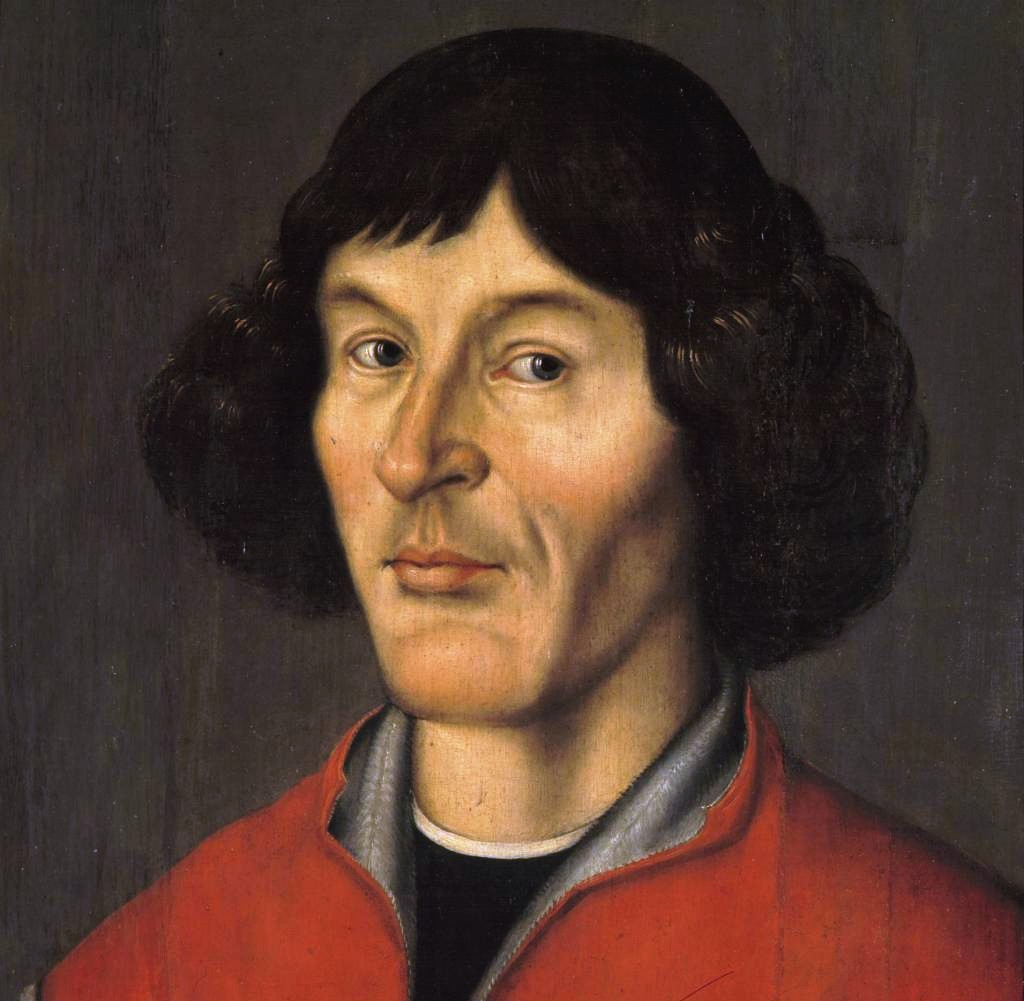
\includegraphics[width=0.618\linewidth]{Kopernik.jpg}
	\caption{Powtórzony rysunek dla testu ciągłości numeracji}
	\label{rys:kopernik2}
\end{figure}

\begin{table}[!b]
 \centering
  \begin{tabular}{p{2.5cm}c|l}
    Data        &   Godzina (UTC)   &   Zdarzenie\\\hline
    2016-05-09  &   14:57           &   Tranzyt Merkurego\\\hline
    2017-08-11 --~2017-08-13  & --- &   Maksimum Perseidów \\\hline
    2018-07-27  &   20:22           &   Całkowite zaćmienie Księżyca\\\hline
    2019-08-24  &   17:04           &   Koniunkcja Wenus i Mars w odległości - 0°17`\\\hline
    2020-12-21  &   16:00           &   Koniunkcja Jowisz i Saturn w odległości 0°06`
  \end{tabular}
 \caption{\label{tab:zjawiska2}Powtórzona tabelka dla testu ciągłości numeracji}
\end{table}

\begin{equation}
    \frac{\partial^2 y}{\partial x^2} = \frac{\mu}{F} \; \frac{\partial^2 y}{\partial t^2}
\end{equation}

\begin{lstlisting}[language=Python,
    caption={Powtórzony kod dla testu ciągłości numeracji},
    label={lst:hello2}]
#!/usr/bin/env python
# -*- coding: utf-8 -*-
"""Simple world of hello.
"""

import sys

def main():
    """The one and only function"""
    fib = lambda n: reduce(lambda x, n: [x[1], x[0]+x[1]], range(n), [0, 1])[0]
    try:
        print(fib(int(sys.argv[1])))
    except:
        print("Hello World!")

if __name__ == "__main__":
    main()
\end{lstlisting}


% Przykładowy wypełniacz
\bredzenie{21-40}


\chapter{Podsumowanie}
\label{ch:podsumowanie}
\chapter{Podsumowanie wyników i wnioski}
\label{ch:podsumowanie}


